\documentclass[a4paper, 12pt]{extarticle}

\usepackage[all]{xy}
\usepackage{amsmath,amsfonts,amssymb}
\usepackage{array}
%\usepackage[backend=biber, style=numeric, sorting=none]{biblatex}
\usepackage{booktabs}
\usepackage{cmap}  % Поддержка поиска русских слов в PDF (pdflatex)
\usepackage{float}
\usepackage{fontawesome}
\usepackage[footnotesize]{caption2}
\usepackage{fullpage}
\usepackage{geometry}
\usepackage{graphicx}
\usepackage[hidelinks]{hyperref}
\usepackage{hyphenat}
\usepackage{indentfirst}
\usepackage{listings}
\usepackage{mathrsfs}
\usepackage{mathtools}
\usepackage{multirow}
\usepackage[ruled,vlined,linesnumbered,algo2e]{algorithm2e}
\usepackage[russian]{babel}
\usepackage{setspace}
\usepackage{theorem}
\usepackage[T2A]{fontenc}
\usepackage[utf8]{inputenc}
\usepackage{verbatim}
\usepackage{vmargin}
\usepackage{xcolor}

\setpapersize{A4}
\setmarginsrb{15mm}{20mm}{15mm}{20mm}{0pt}{0mm}{0pt}{13mm}
\linespread{1.2}

\begin{document}
	\thispagestyle{empty}
	\begin{center}
		Федеральное государственное автономное образовательное учреждение высшего образования
		\\
		\textbf{НАЦИОНАЛЬНЫЙ ИССЛЕДОВАТЕЛЬСКИЙ УНИВЕРСИТЕТ}
		\\
		\textbf{\guillemotleft ВЫСШАЯ ШКОЛА ЭКОНОМИКИ\guillemotright}
		\\[5mm]
		\textbf{Факультет компьютерных наук}
		\\[40mm]
		\textbf{КУРСОВАЯ РАБОТА}
		\\
		\textbf{Методы повышения разнообразия в системах машинного перевода}
		\\[10mm]
		по направлению подготовки Прикладная математика и информатика
		\\
		образовательная программа <<Науки о данных>>
		\\[30mm]
	\end{center}
	\begin{flushright}
		Выполнил:
		\\
		Студент группы мНОД19-АИД-П
		\\
		Солоткий Михаил
		\\[5mm]
		Руководитель:
		\\
		Доцент, кандидат физико-математических наук,
		\\
		Бабенко Максим Александрович
		\\[30mm]
	\end{flushright}
	\vfill
	\begin{center} Москва 2020 \end{center}

\newpage
\renewcommand{\contentsname}{Содержание}
\tableofcontents

\newpage
\begin{abstract}
	В данной работе исследуются методы повышения разнообразия текстов, которые генерируются системами нейросетевого машинного перевода. Приводится сравнение различных методов предложенных ранее в статьях, а также авторских подходов. Приводятся некоторые метрики качества, разработанные для данной задачи.
\end{abstract}

\section*{Введение}
    В области машинного перевода, которые заключается в генерации по заданному тексту на одном естественном языке эквивалентного ему текста на другом естественном языке, в последнее время преобладают нейросетевые подходы. Обычно токены целевого языка генерируются один за другим в том порядке, в котором они будут входить в последовательность. При обучении подобных систем решается задача максимизации логарифма правдоподобия, при этом она решается авторегрессионно. Это значит, что на каждом шаге оценивается вероятность текущего токена при условии всех раннее сгенерированных, а также входной последовательности на исходном языке. При генерации с помощью алгоритма beam search происходит приближённый поиск последовательности, которая максимизировала бы условную вероятность сгенерированной последовательности при условии исходной. При таком подходе мы всегда будем получать единственный перевод исходной последовательности, хотя она могла бы быть корректно переведена множеством разных способов.

    В условиях имеющейся хорошо обученной модели машинного перевода задача состоит в разработке метода генерации разнообразных переводов, которые при этом могли бы сравниться по качеству с наиболее вероятными переводами.

    Также предлагаются автоматически вычисляемые метрики качества для этой задачи, исследуется их адекватность с точки зрения совпадения с человеческими субъективными оценками разнообразия и качества текстов.

\newpage
\section{Нейросетевой машинный перевод}
    Теоретической основной для машинного перевода является вероятностный взгляд на задачу. Во всех известных автору статьях по машинному переводу оперируют с вероятностным распределением $$p \, (\bold{y}  |  \bold{x}) = p \, (y_1  |  \bold{x} ) \, \prod\limits_{t=2}^n \, p \, (y_t | \, y_1, \dots, y_{t - 1}, \bold{x} ) = \prod\limits_{t=1}^n \, p \, (y_t | \, \bold{y}_{< t}, \bold{x} )$$ где $\bold{x} = \{x_1, \dots, x_m\}$ -- входное предложение на исходном языке, $\bold{y} = \{y_1, \dots, y_n\}$ -- предложение на целевом языке. Обучающая выборка обычно состоит из пар $\{ \bold{x}, \bold{y} \}$, где $\bold{y}$ -- перевод предложения $\bold{x}$. При этом не исключается возможность вхождения одного и того же $\bold{x}$ в несколько разных пар $\{ \bold{x}, \bold{y} \}$, то же самое про $\bold{y}$. Что соответствует действительности -- у одного предложения может быть разных одинаково эквивалентных перевода. Это задача обучения с учителем. Существуют и другие постановки, где нет полной разметки, но мы не будем касаться таких постановок.

    Далее это вероятностное распределение приближается некоторой моделью и решается задача максимума правдоподобия. В случае нейросетевого машинного перевода используется энкодер-декодер архитектура: энкодер принимает на вход $\bold{x}$, а декодер принимает на вход $\bold{y}$ и возвращает вероятность $p \, (\bold{y} \, | \, \bold{x})$. Если мы рассматриваем задачу авторегрессионного машинного перевода, то декодер способен выдавать $\forall \, t: 1 \leq t \leq n(\bold{y})$ вероятность $p \, (y_t \, | \, \bold{y}_{< t}, \bold{x} )$.

    Одной из метрик качества перевода (наряду с лог-правдоподобием) является метрика BLEU \cite{bleu}. Она вычисляется как среднее геометрическое точности (precision) по n-граммам, где от 1 до 4 включительно, умноженное на дисконтирующий коэффициент (brevity penalty), который штрафует за слишком длинные переводы. $$\textrm{BLEU}(out, ref) = \min \Bigg\{ 1, \exp \Big\{ \frac{\textrm{len}(ref)}{\textrm{len}(out)} \Big\} \Bigg\} \Big[ \prod\limits_{i=1}^4 \textrm{precision}_i \Big]^{\frac{1}{4}}$$
Точность по n-граммам считается следующим образом -- берётся доля тех n-грамм правильного ответа (reference), которые есть в переводе (output). Очевидно, что всегда можно выдавать перевод, в котором есть всевозможные n-граммы длины от 1 до 4 и получать наивысший precision, но такой перевод будет очень длинный и за счёт дисконтирующего множителя итоговый BLEU получится очень низкий. В случае, если для одного исходного предложения в обучающем наборе имеется несколько переводов, считают максимальный BLEU по всем правильным ответам. То есть если наша версия перевода близка к хотя бы одному reference переводу, это хорошо. BLEU неплохо коррелирует с человеческими субъективными оценками качества перевода. Также есть много критики этой метрики \cite{bleu-critics}, в первую очередь потому что она никак не учитывает смысл предложений, а только слова, с помощью которых оно переводилось. Однако чего-то, что было бы принципиально лучше BLEU пока что не было предложено, насколько известно автору.

    У задачи максимума правдоподобия есть некоторый эффект, который вообще говоря неприятный, если мы хотим хорошо переводить, но полезный в случае, если мы хотим генерировать разнообразные переводы. А именно если в нашем датасете для одного и того же $\bold{x}$ есть несколько разных $\bold{y}$, то есть $\bold{y}_1, \dots, \bold{y}_k$, то оптимальная модель будет стараться предсказывать в некотором смысле среднее ответов $\bold{y}_1, \dots, \bold{y}_k$ в некотором векторном пространстве. Это легко увидеть, записав задачу максимума правдоподобия для набора $\Big\{ \{ \bold{x}, \bold{y}_1 \}, \dots, \{ \bold{x}, \bold{y}_k \} \Big\}$. Обозначим $w_i = p(\bold{y}_i | \bold{x})$.
    $$\sum_{i=1}^k \log w_i \rightarrow\max \;\;\;\;\; w_i \geq 0 \;\;\;\;\; \sum_{i=1}^k w_i \leq 1$$
    Решением будет $w_i = \frac{1}{k}$. Получается, что мы не выучиваем один из правильных ответов, а выучиваем нечто среднее между правильными ответами, что вообще говоря правильным ответом может не являться. Этот эффект можно попытаться убрать, используя другую функцию для оптимизации, например средний BLEU. И обычно на эту функцию дообучают \cite{GNMT} модель, обученную сперва максимизировать правдоподобие, но в наших дальнейших экспериментах это не нужно и делаться не будет.

    Имея обученную модель у нас есть доступ к $p(\bold{y} | \bold{x})$ и можно было бы попробовать из этого распределения взять семпл. Однако на практике такие примеры часто оказываются довольно низкого качества. Если модель недообучена (что правда почти всегда для современных моделей машинного перевода), вероятности восстановлены не совсем правильно, их надо калибровать \cite{calibration}. Мы бы хотели получать не произвольные примеры (среди которых примеры плохого качества могут попадаться довольно часто), а хорошие примеры. Для этого при генерации примеров приближённо ищется $\arg\max\limits_{\bold{y}} p \, (\bold{y} \, | \, \bold{x})$.

    Для авторегрессионной модели генерацию $\bold{y}$ можно производить последовательно по одному токену, при этом для приближённого поиска максимума обычно используется алгоритм beam search. Обычно размер beam небольшой, к примеру, 4 \cite{analyzing-uncertainty}. Алгоритм выдаёт $k$ наиболее вероятных различных (в приближённом смысле) переводов.

\section{Мотивация для разнообразия}
    Разнообразные переводы могут носить разный смысловой или стилистический оттенок. Для изучающих язык (обычно носители обоих языков не переводят с помощью сервисов машинного перевода) это может ускорить процесс их обучения. Или человек хочет сформулировать как-то красиво фразу на другом языке, но не знает, как. Какими бы ни были цели людей, пользующихся машинным переводом, у них появляется возможность выбрать один перевод из набора, который им больше подходит. В классическом подходе, в котором выдаётся один перевод в ответ на запрос, такой возможности выбора нет.

\section{Оценка качества и разнообразия}
    Наиболее точный способ узнать о качестве -- попросить большое количество людей оценить переводы. Можно ввести некоторую шкалу оценок или задавать соответствующие вопросы, например "полностью ли передан смысл исходного предложения". Также можно оценивать разнообразие. Этот способ трудозатратный, хотелось бы иметь автоматически вычисляемые метрики.
    Для автоматического вычисления качества предлагается использовать BLEU. Разве что, он не приспособлен к сценарию, когда предлагается много переводов-кандидатов и полученные BLEU надо как-то агрегировать. Предлагается рассмотреть $\min \textrm{BLEU}$, $\textrm{avg} \, \textrm{BLEU}$ (средний BLEU) и $\max \textrm{BLEU}$. Все три метрики имеют определённый смысл. Средний BLEU показывает качество наших переводов в среднем. Также, как и раньше для оценки качества бралось среднее по датасету, только теперь можно считать, что мы ещё и семплируем датасеты и по ним усредняем. Максимальный BLEU может показывать удовлетворённость человека поиском подходящего ему перевода. В описанном в мотивационной части сценарии предполагается, что пользователь сервиса сможет отбросить все переводы, не подходящие ему и будет судить о качестве системы по её лучшим переводам. Однако, пользователь действительно сможет оценить систему таким образом, если он довольно хорошо знает оба языка. В случае, если он начинает изучать язык, наша система может сгенерировать плохой перевод, что может сбить пользователя с толку и ввести в заблуждение. Поэтому ещё оценивается минимальные BLEU.

    Для вычисления разнообразия предлагается использовать self-BLEU \cite{self-bleu}. Имея $m$ переводов, self-BLEU считается как среднее BLEU по всем парам из этих m переводов. То для каждой пары переводов первый бывает в роли правильного ответа, второй -- кандидата и наоборот. $$\textrm{self-BLEU}(outs) = \frac{1}{\textrm{len} \, (outs) \, ^2} \sum\limits_{i=1}^m \sum\limits_{j=1}^m \textrm{BLEU} (outs_i, outs_j )$$. Эта мера хорошо себя зарекомендовала в статье, в которой была предложена, потому и была выбрана. Ну а так как self-BLEU -- скорее метрика сходства, чем разнообразия и принимает значения от 0 до 1, можно рассмотреть метрику $1 - \textrm{self-BLEU}$.

    Хотелось бы максимизировать все метрики сразу, для этого в экспериментах будут искаться Парето-оптимальные методы с точки зрения всех метрик.

\section{Постановка экспериментов}
\subsection{Архитектура}
    В экспериментах далее использовалась архитектура transformer big -- разновидность transformer, который является лучшей по качеству нейросетевой архитектурой для задачи машинного перевода \cite{attention}.

\subsection{Данные}
    В статьях обычно сравнивают результаты на датасете WMT, который обновляется каждый год. В дальнейших экспериментах использовался датасет WMT'18, исходный язык английский, целевой -- русский. Сеть обучалась на закрытых данных, поэтому с целью сохранения конфиденциальности не будут показываться абсолютные значения BLEU, а только относительные. То есть будет взято некоторое опорное значение BLEU, и все остальные результаты BLEU, которые будут указываться на графиках будут поделены на это опорное значение.

\subsection{Количество переводов}
    Также надо определиться с количеством переводов, выдаваемых разными методами вывода. Дело в том, что обозначенные выше метрики будут сильно зависеть от количества переводов и сравнивать значения этих метрик при разном количестве переводов вообще говоря некорректно -- увеличение показаний было бы вызвано не более качественным алгоритмом, а просто увеличением числа переводов. Например, при подсчёте максимального BLEU среди переводов, увеличивая количество переводов мы неизбежно будем получать более высокие или иногда такие же значения.

    Оказывается, что несмотря на то, что конкретные числа при разном числе переводов будут разные, форма графиков не сильно зависит от количества переводов, если это количество больше одного. Соответственно результаты дальше будут приводиться только для одного конкретного количества переводов, которое было удобно использовать в приложениях данной системы, а именно три.

\section{Методы семплинга}
\subsection{Beam search}
    Для начала стоит измерить результат beam search, а именно средний BLEU, получаемый при выводе трёх переводов. Это значение будет опорным (о котором говорится в секции про постановку экспериментов).

\subsection{Температурный семплинг}
    Оказывается, что переводы, получаемые как $k$ наиболее вероятных в beam search, сильно похожи друг на друга, отличаются примерно в одном слове. Это довольно однообразные примеры. Семплы из распределения $\bold{y}$ получаются низкого качества предположительно потому что переводы плохого качества имеют достаточно большую вероятность. Идея заключается в перевзвешивании вероятностей, получаемых из softmax посредством введения температуры: $$\textrm{softmax}_i(\bold{z}; t) = \textrm{softmax}_i \Big( \frac{\bold{z}}{t} \Big) = \frac{\exp(z_i \, / \, t)}{\sum\limits_{j=1}^n \exp(z_j \, / \, t)}$$ Очевидно, что стоит брать температуру ниже 1 для повышения качества. Ниже приведены графики со всеми заявленными метриками при разных значениях температуры.

\begin{center}
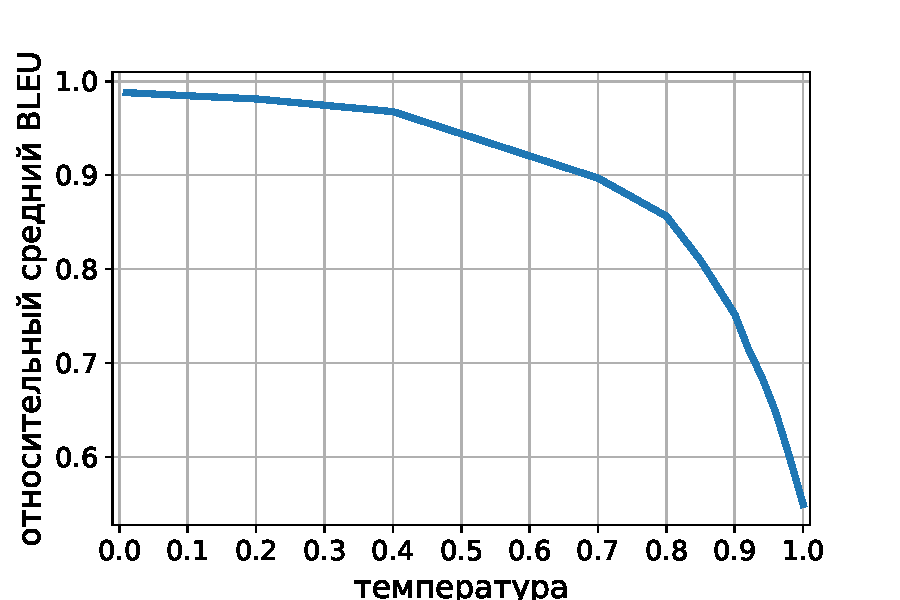
\includegraphics[scale=0.5]{avg-bleu-temperature-sampling.pdf}
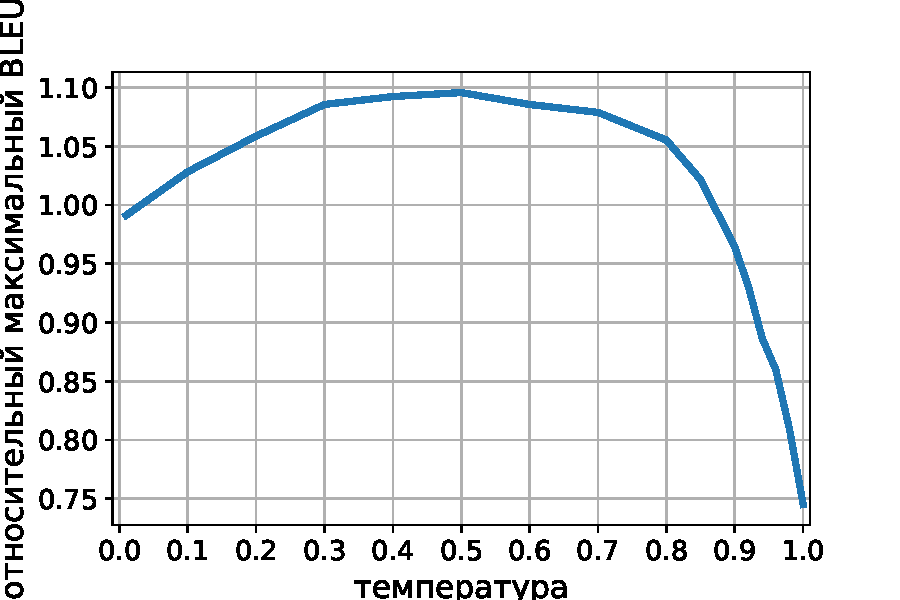
\includegraphics[scale=0.5]{max-bleu-temperature-sampling.pdf}
\end{center}

\begin{center}
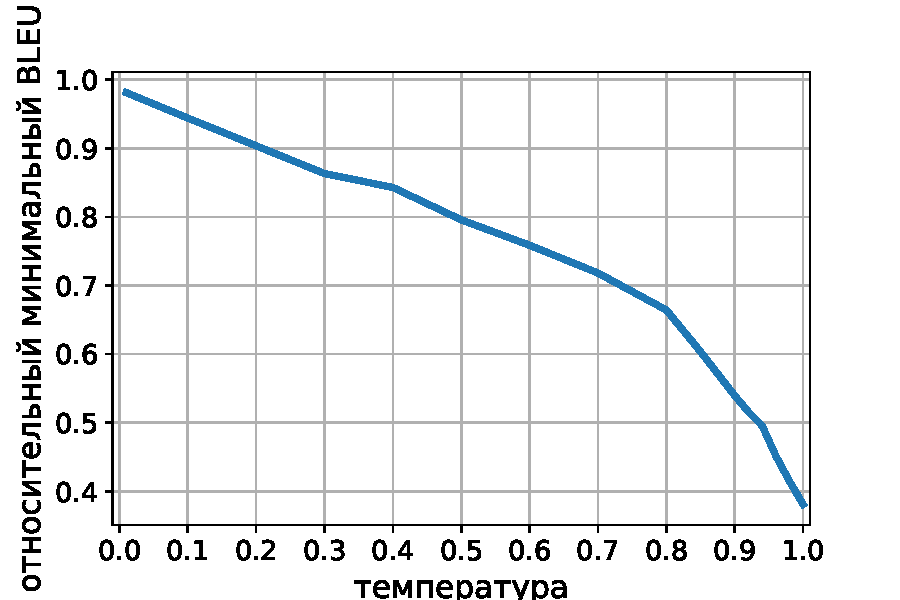
\includegraphics[scale=0.5]{min-bleu-temperature-sampling.pdf}
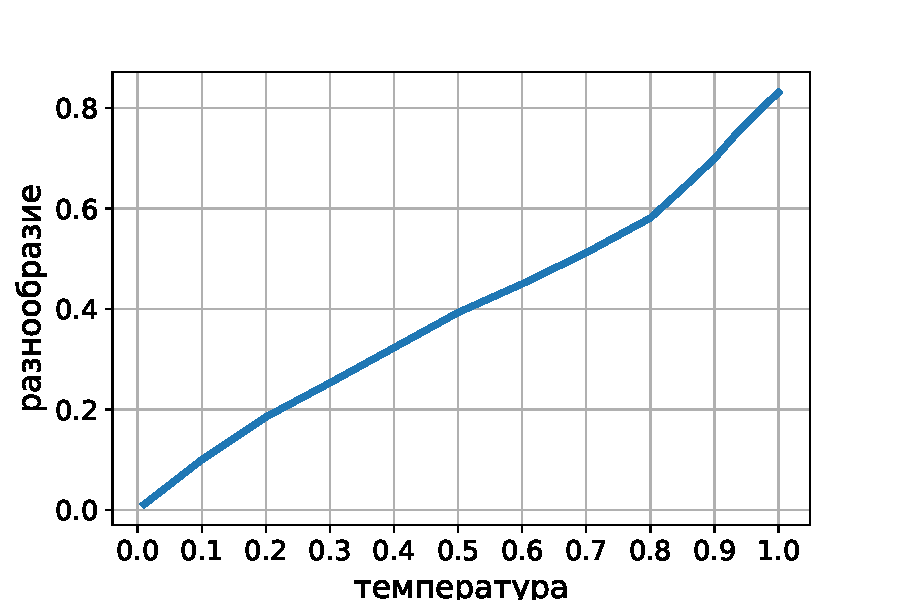
\includegraphics[scale=0.5]{diversity-temperature-sampling.pdf}
\end{center}

Видно, что при температуре близкой к 1 все метрики качества переводов становятся низкими, что на количественном уровне подтверждает наблюдение, что при семплинге переводы получаются плохого качества. Ещё можно заметить, что у максимального BLEU есть локальный максимум около значения 0.5. То есть получается, что за счёт небольшого шума можно получать чуть более качественные переводы наряду с менее качественными, но при большом уровне шума мы уже не способны находить более хорошие переводы. В некотором смысле повышать температуру сильно выше 0.5 не имеет смысла, если цель -- повысить качество, имеет смысл только для увеличения разнообразия.

\subsection{Nucleus sampling}
Идея вдохновлена явлением так называемой деградации текста. Иногда при его последовательном семплировании: начиная с некоторого момента токены в тексте зацикливаются. В статье \cite{nucleus-sampling} исследуются причины этого явления и утверждается, что так происходит из-за того, что вероятности токенов оценены не точно, и некоторые токены, которые должны иметь нулевую вероятность, на самом деле имеют малую вероятность, но её достаточно, чтобы довольно часто такие токены генерировались. В тот момент когда один такой невероятных токен генерируется дальнейшее распределение в при условии уже сгенерированного префикса совсем не соответствует реальному распределению $p \, (\bold{y}_{>t} \, | \, \bold{y}_{\leq t}, \bold{x})$. Соответственно стоит занулить токены с низкой вероятностью для избежания такого явления, перенормировать оставшиеся вероятности и далее можно так же делать семплинг. Идея называется nucleus sampling. По сравнению с обычным семплингом в nucleus sampling появляется новый параметр $p$ -- вероятностная масса, которую необходимо отбросить. Температура в методе, как и в оригинальной статье равна 1. Ниже приведены графики метрик при разном значении $p$.

\begin{center}
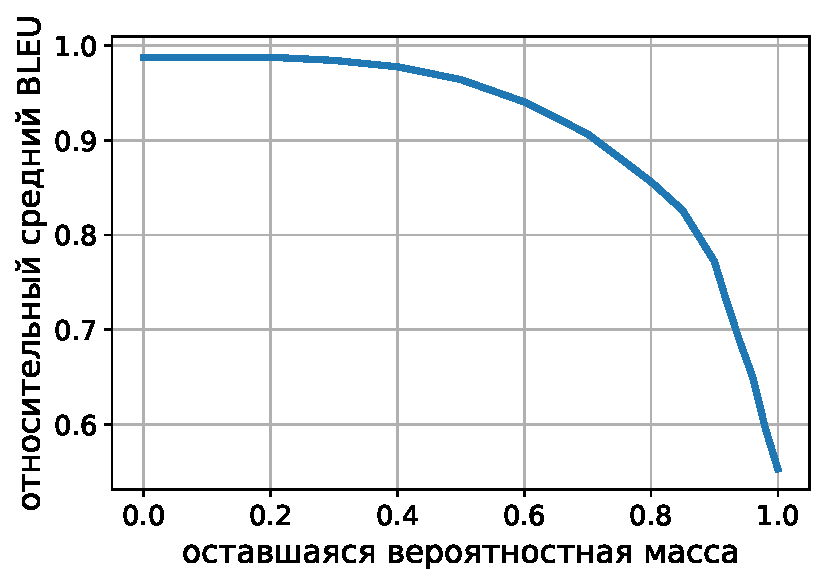
\includegraphics[scale=0.5]{avg-bleu-nucleus-sampling.pdf}
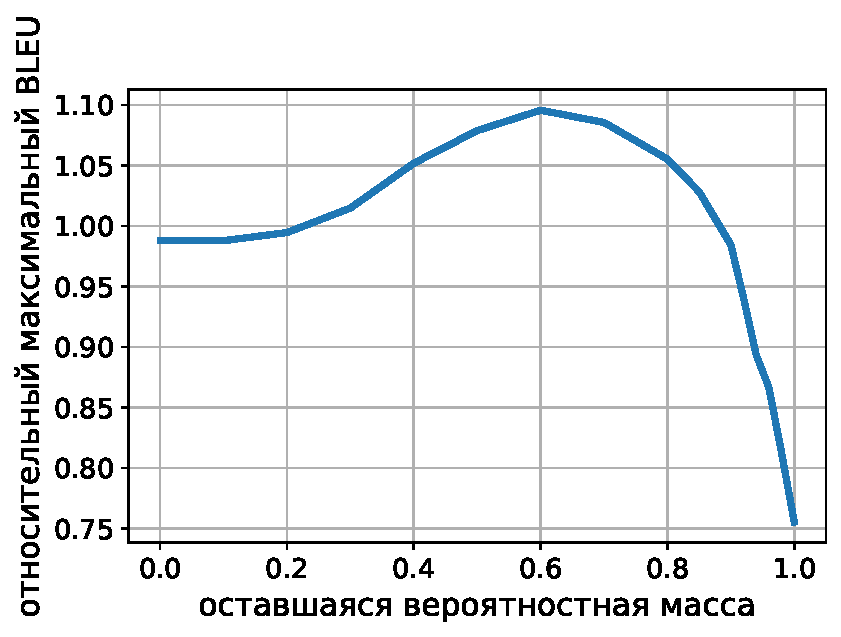
\includegraphics[scale=0.5]{max-bleu-nucleus-sampling.pdf}
\end{center}

\begin{center}
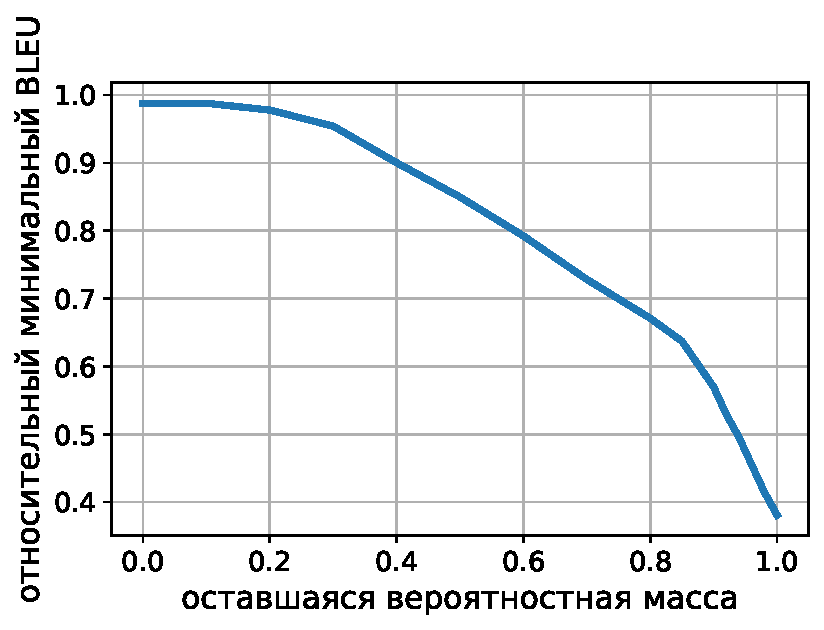
\includegraphics[scale=0.5]{min-bleu-nucleus-sampling.pdf}
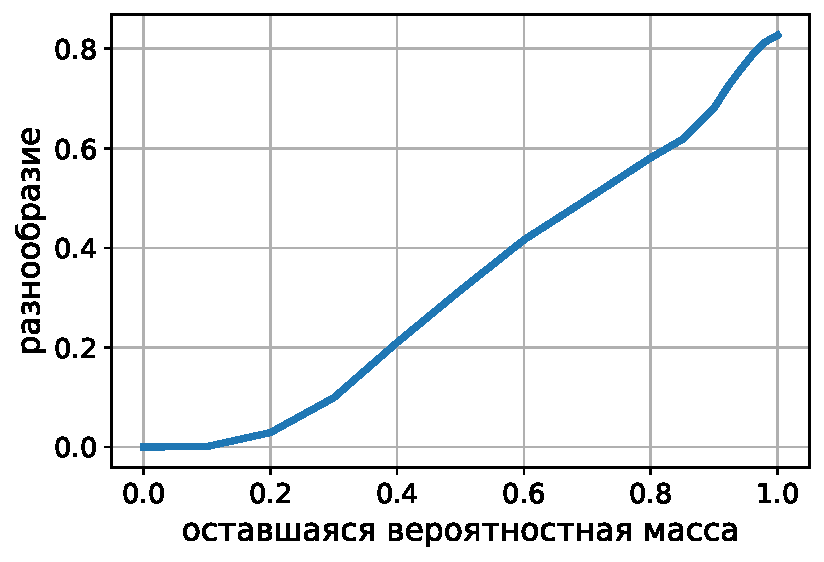
\includegraphics[scale=0.5]{diversity-nucleus-sampling.pdf}
\end{center}

Абсолютные значения примерно такие же, разве что форма графиков немного поменялась.

\subsection{Diverse resampling}
    Следующая идея авторская -- diverse resampling. Суть в том, что уровень разнообразия, получаемый некоторым методом зависит от исходного предложения. Некоторые предложения тяжелее перевести тремя разными способами, чем другие. Идея в том, чтобы сгенерировать с помощью некоторого метода семплинга некоторое большое количество переводов и среди них выбрать три наиболее далёких друг от друга. Этот подход требует гораздо больше ресурсов, чем предыдущие, так как получается, что некоторые переводы генерировались напрасно и просто отбрасываются, однако с помощью него можно получать потенциально более разнообразные переводы, не увеличивая температуру, то есть не ухудшая явно качество.

    В эксперименте семплировалось (с температурой) 10 переводов, далее брался лучший (по лог-правдоподобию) перевод, после него находился самый далёкий по self-BLEU перевод от него, найденный перевод становился вторым в выдаче, и третий перевод находился как наиболее далёкий по self-BLEU к выбранным ранее двум переводам.

    Подход не сработал, средний, максимальный и минимальные BLEU уменьшились на несколько единиц при незначительном улучшении разнообразия. При сравнении с другими методами оказался Парето-неоптимальным. Это теоретически могло произойти потому, что бралось много семплов из распределения, получаемое из нейросети, которое восстановлено неидеально, а затем из этого распределения выбирались специально далёкие (в смысле self-BLEU переводы).

\subsection{Diverse beam search}
В статье \cite{diverse-beam} был предложен метод diverse beam search. Там решалась проблема повышения разнообразия в задаче image captioning и немного было также о повышении разнообразия в машинном переводе. У авторов были другие метрики и не было сравнения с другими методами генерации разнообразных переводов. Метод заключается в последовательном использовании beam search. Первый раз происходит вывод с обычным beam search. Во второй и последующий разы к функционалу, который максимизируется в beam search, добавляется член, стимулирующий разнообразие $$\ln p \, (y_t \, | \, \bold{y}_{<t}, \bold{x}) + \sum_{i=1}^{k - 1} \lambda_i \, \textrm{div}(\bold{y}_{\leq t}, \, \bold{y}^i) \rightarrow \max\limits_{y_t}$$ где $k$ -- номер группы, к которой относится генерируемое сейчас предложение. Речь идёт о группах переводов, так как beam search выдаёт один или больше наиболее правдоподобных переводов. Здесь берётся сумма некоторой метрики разнообразия с раннее сгенерированными переводами. При этом из каждой группы берётся один перевод -- самый лучший. То есть группы имеют смысл только на этапе генерации, когда она завершается -- от группы остаётся один перевод.

    В качестве функции div использовалась та самая метрика разнообразия, с помощью которой это разнообразие предлагалось мерять. Использование в оптимизации той же самой метрики, с помощью которой оценивается качество может показаться нечестным преимуществом. К примеру, можно сказать, что именно поэтому удалось получить высокое качество наряду с разнообразием, а не потому что метод лучше исследует пространство гипотез. Как метод себя бы вёл в условиях, когда нет возможности оптимизировать ту же самую метрику, с помощью которой оценивается качество, неизвестно -- такие эксперименты не проводились. В работе ставится акцент на то, что доступ к этой самой метрике есть, и этим метод на качественном уровне лучше того же температурного семплинга, так как в последнем напрямую не оптимизируется некая произвольная метрика разнообразия.

    Описанный метод последовательный, то есть предполагает полное завершение генерации текущей группы переводов для начала генерации следующей. При этом self-BLEU можно считать и на префиксах переводов, а значит параллельно осуществлять вывод гипотез в разных группах. При этом можно поддерживать гипотезы одинаковой длины (либо отличающейся на 1 в момент генерации нового токена) и постепенно добавлять по одному токену к каждой.

    Коэффициент лямбда для разных групп можно делать разным, однако в наших экспериментах более тщательный подбор разных лямбд не дал заметного улучшения по сравнению с режимом, где лямбда одна и та же для всех групп. Графики метрик в зависимости от коэффициента лямбда получаются по форме и абсолютным значениям примерно такие же, как для предыдущих методов вывода. Ниже приведены графики сравнения с предыдущими методами в осях разнообразие, агрегированный BLEU.

\begin{center}
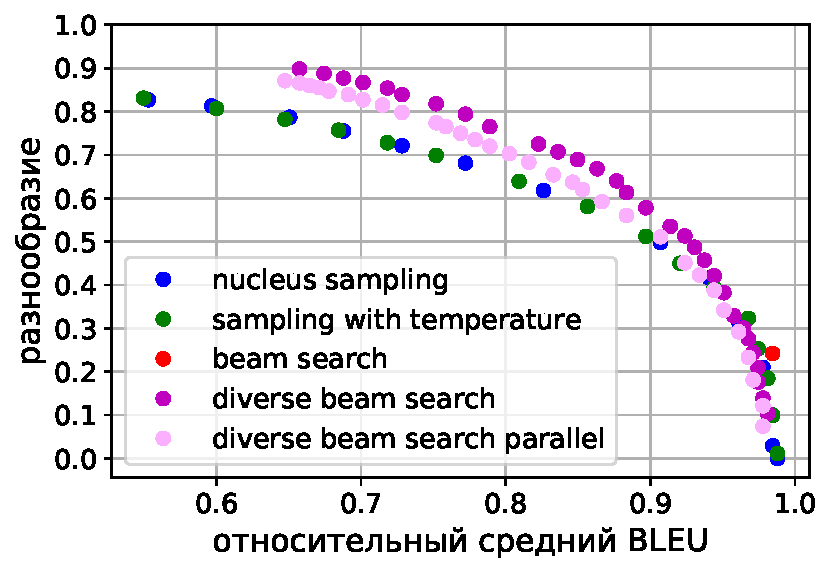
\includegraphics[scale=0.5]{avg-bleu-diverse-beam-search.pdf}
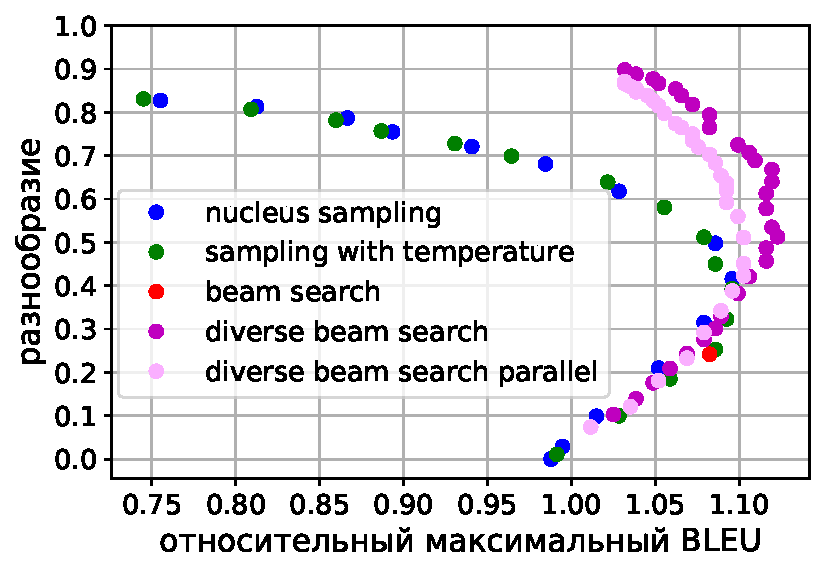
\includegraphics[scale=0.5]{max-bleu-diverse-beam-search.pdf}
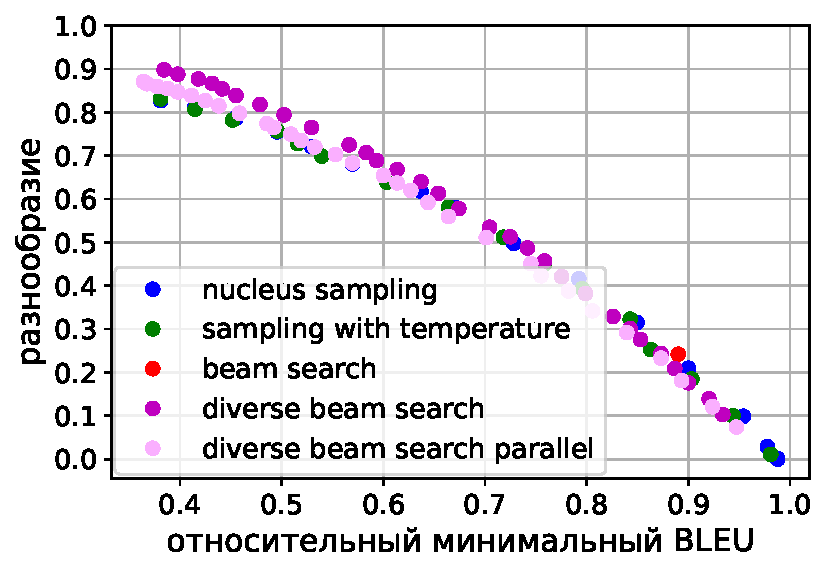
\includegraphics[scale=0.5]{min-bleu-diverse-beam-search.pdf}
\end{center}

Видно, что по всем метрикам подход diverse beam search обгоняет предыдущие подходы. При этом даже удалось повысить максимальное качество и при одном и том же уровне качества (будь то средний BLEU, минимальный или максимальный, разнообразие переводов получилось выше). У этого подхода есть некоторый недостаток -- генерация трёх примеров при том, что в каждой группе по, допустим, две гипотезы, эквивалентна по затраченному времени шести прогонам сети, что либо дольше трёх прогонов, либо требует больше ресурсов для параллельной генерации. Параллельная версия, кстати, даёт не самый лучший результат в соотношении качество -- разнообразие, её результаты Парето-неоптимальны. Возможно, дело в том, что при для генерации отличного от данного перевода нужна информация о переводе целиком, а не только префикс той же длины.

\section{Примеры переводов}
    Кроме численных метрик, проводилась субъективная оценка качества переводов автором: бралось небольшое количество исходных предложений и генерировалось по несколько переводов для методов температурного семплинга, nucleus sampling и diverse beam search. Качество каждого сгенерированный перевода оценивалось по тернарной шкале: <<хорошо>>, <<плохо>>, <<не уверен>>.

\begin{center}
    \begin{tabular}{c|c|c|c|}
        \cline{2-4}
        & nucleus sampling, p = 0.5 & темп. семплинг, t = 0.7 & diverse bs, $\lambda = 10.0$ \\ \cline{1-4}
        \multicolumn{1}{|c|}{<<хорошо>>} & 64 / 120 & 52 / 120 & 20 / 36 \\ \cline{1-4}
        \multicolumn{1}{|c|}{<<плохо>>} & 34 / 120 & 42 / 120 & 5 / 36 \\ \cline{1-4}
        \multicolumn{1}{|c|}{<<не уверен>>} & 22 / 120 & 26 / 120 & 11 / 36 \\ \cline{1-4}
    \end{tabular}
\end{center}

Также есть примеры работы методов. Предложение <<As a coach, I would tell you it's time to run another play.>>\\

Diverse beam search переводит так: \\
1) Как тренер, я бы сказал вам, что пришло время запустить другую игру.\\
2) Как тренер, скажу тебе, что пора начать новую игру.\\
3) Как тренер, я хочу сказать, что пришло время начать новую игру.\\

Обычный beam search выдаёт:\\
1) Как тренер, я бы сказал вам, что пришло время запустить другую игру.\\
2) Как тренер, я бы сказал вам, что пришло время запустить еще одну игру.\\
3) Как тренер, я хотел бы сказать вам, что пришло время запустить другую игру.\\

Семплинг с температурой t = 0.7 даёт: \\
1) Как тренер, я скажу вам, что пришло время снова сыграть.\\
2) Как тренер, я хотел бы сказать вам, что пришло время провести еще одну игру.\\
3) Как тренер, я бы сказал, что пришло время играть в другой пьесе.\\

\section{Выводы}
    Diverse beam search показал себя лучше остальных методов. Он сочетает в себе максимизацию условной вероятности и разнообразие. В этом его преимущество, к примеру, по отношению к температурному семплингу, кв котором не происходит оптимизации $p\, (\bold{y} \, | \, \bold{x})$. Более того, diverse beam search в отличие от методов семплинга напрямую оптимизирует заданную метрику разнообразия, соответственно есть возможность получить дополнительный прирост только за счёт более точной оптимизации. С помощью параметров $\lambda_i$ можно контролировать качество и разнообразие, также как и в температурном семплинге и nucleus sampling. Можно сказать, что diverse beam search занимается исследованием пространства $\bold{y}(\bold{x})$ и за счёт оптимизации может находить альтернативные формы перевода с высокой вероятностью, сильно отличающиеся от первоначального , что довольно сделать с помощью семплинга.

\section{Результаты}
\begin{itemize}
\item Была введена формализация понятий качества и разнообразия в машинном переводе и показана их адекватность
\item Реализованы и испробованы различные методы генерации разнообразных переводов, в том числе придуманы новые
\item Сделано сравнение методов по времени работы, качеству и разнообразию, а также с точки зрения потребления ресурсов
\item Для лучшего метода -- diverse beam search -- предложена параллельная реализация и адаптация к специально выбранной метрике разнообразия
\end{itemize}

\newpage
\renewcommand{\bibname}{Список литературы}
\addcontentsline{toc}{section}{\bibname}

\def\BibUrl#1.{}\def\BibAnnote#1.{}
\def\BibUrl#1{\\{\footnotesize\tt\def~{\char126} http://#1}}

\bibliographystyle{apalike}
\bibliography{references}

\end{document}